\documentclass[utf8,zihao=-4,a4paper]{ctexart}

\usepackage{xeCJK}
\newcommand{\zhongsong}{\CJKfontspec{STZhongsong}} %华文中宋,请自行下载字体并安装
\newcommand{\xiaosi}{\fontsize{12pt}{18pt}\selectfont}            % 小四, 1.5倍行距
\newcommand{\sihao}{\fontsize{14pt}{21pt}\selectfont}            % 四号, 1.5 倍行距
\newcommand{\xiaosan}{\fontsize{15pt}{22pt}\selectfont}        % 小三, 1.5倍行距
\newcommand{\xingkai}{\CJKfontspec{STXingkai}}
\usepackage{fontspec}
\setmainfont{Times New Roman}


%==================== 数学符号公式 ============
\usepackage{amsmath}                 % AMS LaTeX宏包
\usepackage[ruled]{algorithm2e}              %伪代码
\usepackage{amssymb}                % 用来排版漂亮的数学公式
\usepackage{amsbsy}
\usepackage[style=1]{mdframed}
\usepackage{amsthm}
\usepackage{amsfonts}
\usepackage{mathrsfs}                % 英文花体字 体
\usepackage{bm}                      % 数学公式中的黑斜体
\usepackage{bbding,manfnt}           % 一些图标,如 \dbend
\usepackage{lettrine}                % 首字下沉,命令\lettrine
\usepackage{gbt7714}                 %配置gb7714引用格式
\usepackage{lscape}

\def\attention{\lettrine[lines=2,lraise=0,nindent=0em]{\large\textdbend\hspace{1mm}}{}}
\usepackage{longtable}
\usepackage[toc,page]{appendix}
\usepackage{geometry}                % 页边距调整
\geometry{top=3.5cm,bottom=2.5cm,left=2.5cm,right=2.5cm}
%\usepackage{relsize}                % 调整公式字体大小:\mathsmaller,\mathlarger
%\usepackage{caption2}               % 浮动图形和表格标题样式
\usepackage{booktabs}                %三线表上下加粗
\usepackage{diagbox}                 % 分类表头

\newlength\szg
\newcommand\quan[1]{%
\settoheight\szg{#1}%
\tikz[baseline]{\pgfmathparse{
ifthenelse(#1 < 10, 1, ifthenelse(#1 < 100, 0.75, 0.5))
}
\let\hfs\pgfmathresult
\node at (0,\szg/2) {\makebox[0em][c]{\scalebox{\hfs}[1]{#1}}};
\draw (0,\szg/2) circle (\szg/2+0.35ex);
}}

%====================公式按章编号==========================
\numberwithin{equation}{section}
\numberwithin{table}{section}
\numberwithin{figure}{section}
%================= 基本格式预置 ===========================
\usepackage{fancyhdr}

\pagestyle{fancy}
\fancyhf{}  
\fancyhead[C]{\zihao{5} 河南旅游中心项目安全施工组织设计 }
\fancyfoot[C]{~\zihao{5} -\thepage-~}
\renewcommand{\headrulewidth}{0.65pt} 
\ctexset{
    section = {
        format = \bfseries \zihao{-3} \heiti ,
        name = {, }
    },
    subsection = {
        nameformat = \bfseries \zihao{-4} \heiti
    },
    subsubsection = {
        nameformat = \bfseries \zihao{-4} \heiti
    }
}

%================== 图形支持宏包 =========================
\usepackage{subfigure}
\usepackage{graphicx}                % 嵌入png图像
\usepackage{color,xcolor}            % 支持彩色文本、底色、文本框等
\usepackage{hyperref}                % 交叉引用
\usepackage{caption}
\usepackage{multirow}                  %合并表格
% set up labelformat and labelsep for figure
\captionsetup{labelsep=quad}
\captionsetup{figurewithin=section}

\renewcommand{\thesubfigure}{(\arabic{subfigure})} %还可设置图编号显示格式,加括号或者不加括号

%==================== 源码和流程图 =====================
\usepackage{listings}                % 粘贴源代码
\usepackage{tikz}                    
\usepackage{tikz-3dplot}
\usetikzlibrary{shapes,arrows,positioning}
%===================   正文开始    ===================
\begin{document}
%===================  定理类环境定义 ===================
\newtheorem{example}{例}              % 整体编号
%\newtheorem{algorithm}{算法}
\newtheorem{theorem}{定理}            % 按 section 编号
\newtheorem{definition}{定义}
\newtheorem{axiom}{公理}
\newtheorem{property}{性质}
\newtheorem{proposition}{命题}
\newtheorem{lemma}{引理}
\newtheorem{corollary}{推论}
\newtheorem{remark}{注解}
\newtheorem{condition}{条件}
\newtheorem{conclusion}{结论}
\newtheorem{assumption}{假设}
%==================重定义 ===================
\renewcommand{\contentsname}{目 ~~ 录}     
\renewcommand{\abstractname}{摘 ~~ 要} 
\renewcommand{\refname}{参考文献}     
\renewcommand{\indexname}{索引}
\renewcommand{\figurename}{图}
\renewcommand{\tablename}{表}
\renewcommand{\appendixname}{附录}
\renewcommand{\proofname}{证明}
\renewcommand{\algorithmcfname}{算法} 
%\renewcommand{\algorithm}{算法} 
%============== 封皮和前言 =================
%===============  封面  =================
\smallskip
\begin{center}

\vspace*{2.2cm}
\zhongsong{\zihao{1} 沈阳建筑大学} \\
\vspace*{3.3cm}
\heiti{\zihao{2} 毕业设计 }\\
\vspace*{5.5cm}

\zhongsong
\begin{tabular}{cc}
 \zihao{-2} 毕业设计题目:&\underline{\makebox[7cm][c]{\zihao{-2}毕业设计}} \\ 
 \\
 \zihao{-2}学院专业班级: & \underline{\makebox[7cm][c]{\zihao{-2}土木学院安全工程 1602}} \\ 
 \\
 \zihao{-2}学生姓名: & \underline{\makebox[7cm][c]{\zihao{-2}曲俊宇}} \\ 
 \\
 \zihao{-2}指导教师: & \underline{\makebox[7cm][c]{\zihao{-2}刘家喜}} \\ 
 \\
\end{tabular} 
\end{center}
\thispagestyle{empty}
\clearpage
%=====================原创性声明===========
\begin{center}
\zihao{-2} \textbf{学位论文原创性声明}
\end{center}

本人郑重声明:所呈交的论文是本人在导师的指导下独立进行研究所取得的研究成果。除了文中特别加以标注引用的内容外,本论文不包括任何其他个人或集体已经发表或撰写的成果作品。本人完全意识到本声明的法律后果由本人承担。 
\begin{flushright}
\zihao{4} 作者签名:\qquad ~~~\\

年\qquad 月\qquad 日
\end{flushright}
\vskip 2cm
\begin{center}
\zihao{-2} \textbf{学位论文版权使用授权书}
\end{center}

本学位论文作者完全了解学校有关保障、使用学位论文的规定,同意学校保留并向有关学位论文管理部门或机构送交论文的复印件和电子版,允许论文被查阅和借阅。本人授权省级优秀学士论文评选机构将本学位论文的全部或部分内容编入有关数据进行检索,可以采用影印、缩印或扫描等复制手段保存和汇编本学位论文。\smallskip

本学位论文属于
\begin{tabular}[t]{l}
1、保密$ \Box$,在~~~年解密后适用本授权书  \\ 
2、不保密$ \Box$  \\ 
\end{tabular} \\
\begin{center}
(请在以上相应方框内打“$\surd”$)
\end{center}
\begin{flushright}
\zihao{4} 作者签名:  \quad\quad\quad\quad 年 \quad  月  \quad  日\\
导师签名:   \quad\quad\quad\quad 年 \quad  月 \quad   日\\
\end{flushright}
\thispagestyle{empty}
\clearpage

%%=============设计(论文)任务书===========
\begin{center}
\zihao{-2}\textbf{\songti 本科生毕业设计(论文)任务书} 
\end{center}
\smallskip
\renewcommand{\arraystretch}{1.3}
\begin{tabular}{lll}
\zihao{4} \textbf{\songti 学生姓名: 曹宇} & & \zihao{4} \textbf{\songti 专业班级:\quad\quad 船海1006班} \\ 
\zihao{4} \textbf{\songti 指导教师:徐海祥}&\makebox [3cm] & \zihao{4} \textbf{\songti 工作单位:\quad 武汉理工大学} \\ 
\end{tabular}\\
\begin{tabular}{lll}
\zihao{4} \textbf{\songti 设计(论文)题目:}& \zihao{4} \textbf{\songti  武汉理工本科论文\LaTeX 模板 } &\\ 
\zihao{4} \textbf{\songti 设计(论文)主要内容:} \\
\end{tabular} \\ 
\begin{enumerate}
\item \LaTeX 环境的配置
\item 主要字体的控制和数学公式的选用
\item 图表和代码的粘贴
\end{enumerate}
\begin{tabular}{ll}
\zihao{4} \textbf{\songti 要求完成的主要任务:}
\end{tabular} \\ 
\begin{enumerate}
\item 选择合适的\TeX 编辑系统
\item 学习如何使用控制代码完成排版
\item 合理的安排学习和科研的时间来发展自己兴趣爱好
\end{enumerate}
\begin{tabular}{ll}
\zihao{4} \textbf{\songti 必读参考资料:}
\end{tabular}
\begin{enumerate}
\item \LaTeX  \quad User Manual
\item  字体设计的艺术
\end{enumerate}
\begin{tabular}{lll}
\zihao{4} \textbf{\songti 指导教师签名: }&\makebox [4cm]& \zihao{4} \textbf{\songti 系主任签名:} \\
& & \zihao{4} \textbf{\songti 院长签名(章)}
\end{tabular}
\thispagestyle{empty}
\clearpage
%==========本科生毕业设计(论文)开题报告  =============
\begin{center}
\zihao{-2} \textbf{\songti 武汉理工大学}\\
\zihao{-2} \textbf{\songti 本科生毕业设计(论文)开题报告} 
\end{center}
\begin{tabular}{|l|}
\hline \rule[-2ex]{0pt}{5.5ex} \makebox[13.5cm][l]{\zihao{4} \heiti 1、目的及意义(含国内外的研究现状分析) } \\ 
\quad \LaTeX 是国际通行的科技论文排版软件,国际上科研机构和大学都采用它写作\\
\quad 国内著名高校都有自己的本科生\LaTeX 模板供毕业生使用\\
\quad 但是武汉理工大学还没有本科生\LaTeX 模板可以参考\\
\quad 人类的价值在于创造而不是索取 \\
\hline \rule[-2ex]{0pt}{5.5ex}  \zihao{4} \heiti
2、基本内容和技术方案\\ 
\quad 采用GITHUB托管降低代码维护成本\\
\quad 加入在线\TeX 编辑器的使用简介 \\
\quad 授人以渔,注重方法和理念的引导\\
\hline \rule[-2ex]{0pt}{5.5ex}  \zihao{4} \heiti
3、进度安排 \\ 
\quad 离 deadline 两个月吃喝玩乐 \\
\quad 离 deadline 一个月吃喝玩乐 \\
\quad 离 deadline 半个月吃喝玩乐 \\
\quad 离 deadline 一个星期狂写论文 \\
\hline \rule[-2ex]{0pt}{5.5ex} \zihao{4} \heiti
4、指导教师意见 \\ 
\quad 曹宇同学是个好同志\\
\quad 曹宇同志是个好同学\\
\quad 本表格是支持跨页的长表格,你可以复制上面的内容进行测试\\
\quad 具体方法是将tabular改为 longtable然后再编译\\
\makebox[10cm][r]指导教师签名:\\
\makebox[12cm][r]\quad 年\quad 月\quad 日\\
\hline 
\end{tabular} 
\thispagestyle{empty}

\pagestyle{plain}
\pagenumbering{Roman}
\section*{\zihao{-2} \centering 摘 ~~ 要}

\vskip0.5cm
本设计名称为“X————————————————”,建筑总高度为 95.25m, 建筑层数为 30  层,主要针对该项目的施工过程进行全面的安全方案设计。
通过制定本工程的施工组织设计,了解各个部分工程的基本施工方案,制定评价单元,从而确定施工过程中人的不安全行为和物的不安全状态,
对施工现场中的危险源进行辨识, 运用事故树、预先危害分析、安全检查表等方法对施工现场中存在的危险源进行评价, 对已经发现的危险危害因素做出预防措施,
并且制定相应的应急预案。

本工程属于框架剪力墙结构,其中脚手架工程采用落地式和悬挑式脚手架两种, 搭设高度均为 18.00m;模板工程采用木模板,支模高度为 8.95m 属于高支模;
脚手架及模板支撑体系均采用 Ф48.3×3.6 钢管;基坑达到 9.40m,采用混凝土灌注桩并配有双层锚杆支护方式。均属于超出一定规模的危险性较大的分部分项工程,
风险性极大, 因此本次设计针对以上三部分分别做出了专项方案。

根据 “安全第一,预防为主,综合治理”的安全方针,建立项目安全生产管理组织机构,健全和完善相关管理制度。根据危险源辨识与评价,制定重大事故的相应应急预案,
形成完整的管理责任流程,为项目部安全管理提供完整、高效的管理依据。\\



{\zihao{4} \heiti 关键词: } \zihao{-4}施工组织设计;危险源辨识;安全评价;专项施工方案;应急预案
\addcontentsline{toc}{section}{摘要}

\clearpage
\section*{\zihao{-2} \centering \textbf{Abstract} }
   %用了Times New Roman字体来美化观感

   This design is entitled "XX safety construction or ganization and design", building a total height of 95.25 m, building layer number is 30, 
   mainly for the project construction process to conduct a comprehensive safety plan design. Are formulated by the construction organization design, 
   to understand each part project of basic construction plan, make evaluation unit, to determine the construction process of human uns afe behavior 
   and unsafe state of the content of the construction site of the hazards are identif ied, using the fault tree, preliminary hazard analysis, safety 
   check list method to evaluate th e hazards that exist in the construction site, have found that the risk of harm factors to make preventive measures,
    and formulate the corresponding contingency plans.

   This project belongs to the frame shear wall structure, in which the scaffold project adopts fl oor type and overhanging type of scaffolding, 
   and the height of erection is 18.00m. The for mwork adopts wooden template, and the supporting height is 8.95m. Scaffolding and formw ork 
   supports system adopts Ф 48.3 x 3.6 steel tube; The foundation pit reaches 9.40m, with concrete cast-in-place pile and double-deck anchor 
   bolt support. All of them belong to sub-p rojects with greater risks than a certain scale, which have great risks. Therefore, this design 
   makes special plans for the above three parts respectively.

   According to the safety policy of "safety first, prevention first, comprehensive management ", the project safety production management 
   organization is established, and related manage ment system is improved. According to the identification and evaluation of dangerous sources,
    the corresponding emergency plan for major accidents is formulated to form a complete management responsibility flow, providing a complete 
    and efficient management basis for t he safety management of the project department.
    \\

\textbf{\zihao{4} Key Words:} Construction organization design; Hazard identification; Safety assessment; Special construction plans; The emergency response plan

\addcontentsline{toc}{section}{Abstract}





\tableofcontents 
\begin{center}
    \section*{\zihao{-3}  \textbf{引 ~~ 言}}
\end{center}
\pagenumbering{arabic}

\vskip0.5cm
\zihao{-4}理工文科所有专业本科生的毕业设计(论文)都应有“引言”的内容。如果引言部分省略,该部分内容在正文中单独成章,标题改为文献综述,用足够的文字叙述。从引言开始,是正文的起始页,页码从1开始顺序编排。
针对做毕业设计:说明毕业设计的方案理解,阐述设计方法和设计依据,讨论对设计重点的理解和解决思路。

针对做毕业论文:说明论文的主题和选题的范围;对本论文研究主要范围内已有文献的评述;说明本论文所要解决的问题。建议与相关历史回顾、前人工作的文献评论、理论分析等相结合。

注意:是否如实引用前人结果反映的是学术道德问题,应明确写出同行相近的和已取得的成果,避免抄袭之嫌。注意不要与摘要内容雷同。

书写格式说明:
标题“引言”选用模板中的样式所定义的“引言”;或者手动设置成字体:黑体,居中,字号:小三,1.5倍行距,段后1行,段前为0行。

引言的字数在3000字左右(毕业设计类引言可适当调整为800字左右)。引言正文选用模板中的样式所定义的“正文”,每段落首行缩进2字;或者手动设置成每段落首行缩进2字,宋体,小四,多倍行距 1.25,段前、段后均为0行,取消网格对齐选项。
\addcontentsline{toc}{section}{引言}
\pagestyle{fancy}

%============== 论文正文   =================
\pagestyle{fancy}

\section{工程概况}
\subsection{施工组织设计编制基本原则}

施工组织设计按照编制对象,可分为施工组织总设计、单位工程施工组织设计。
施工组织设计应包括编制依据、工程概况、施工部署、施工准备与资料配置计划、
施工进度计划、主要施工方法、施工管理措施、施工现场平面布置等主要内容;
施工组织设计的编制必须遵循工程建设程序,并符合下列原则:

\begin{itemize}

    \item [1)] 符合国家有关法律法规、现行规范,符合地方规程、行业标准的要求;

    \item [2)] 满足建筑施工合同或招标文件中关于建筑工程进度、质量、环境保护、职业健康、安全、工程造价等工程管理目标的要求;

    \item [3)] 积极开发、推广运用新技术、新工艺、新材料、新设备;

    \item [4)] 坚持科学的施工程序和合理的施工顺序,做到资源的优化组织和合理配置,采用流水施工和网络计划的方法,实现均衡施工,努力实现科学、合理的经济技术指标;

    \item [5)] 积极响应国家关于低碳、节能、环保方面的方针、政策;采取先进的技术和管理措施,推广建筑节能和绿色施工。

    \item [6)] 与建筑施工单位质量、环境、职业健康安全、项目管理规范四合一标准的有效结合,贯彻质量、环境、职业健康安全管理国家管理规范的要求;

\end{itemize}

\subsection{施工组织设计编制程序}

施工组织设计的编制程序应遵守如下流程:

(1)收集和熟悉编制施工组织总设计所需的有关资料和图纸,进行项目特点的施工条件的调查研究;

(2)计算主要工种工程的工程量;

(3)确定施工的总体部署;

(4)拟定施工方案;

(5)编制施工总进度计划;

(6)编制资源需求量计划;

(7)编制施工准备工作计划;

(8)施工总平面图设计;

(9)计算主要技术经济指标。应该指出以上顺序中有些顺序必须固定,不可逆转,如:

\quan{1} 拟定施工方案后才可编制施工总进度计划(因为进度的安排取决于施工的方案);

\quan{2} 编制施工总进度计划后才可编制资源需求量计划(因为资源需求量计划要反映各种资源在时间上的需求)

施工组织设计的编制程序流程图见图 \ref{fig:c1f1}

\begin{figure}[thbp!]
    \centering
    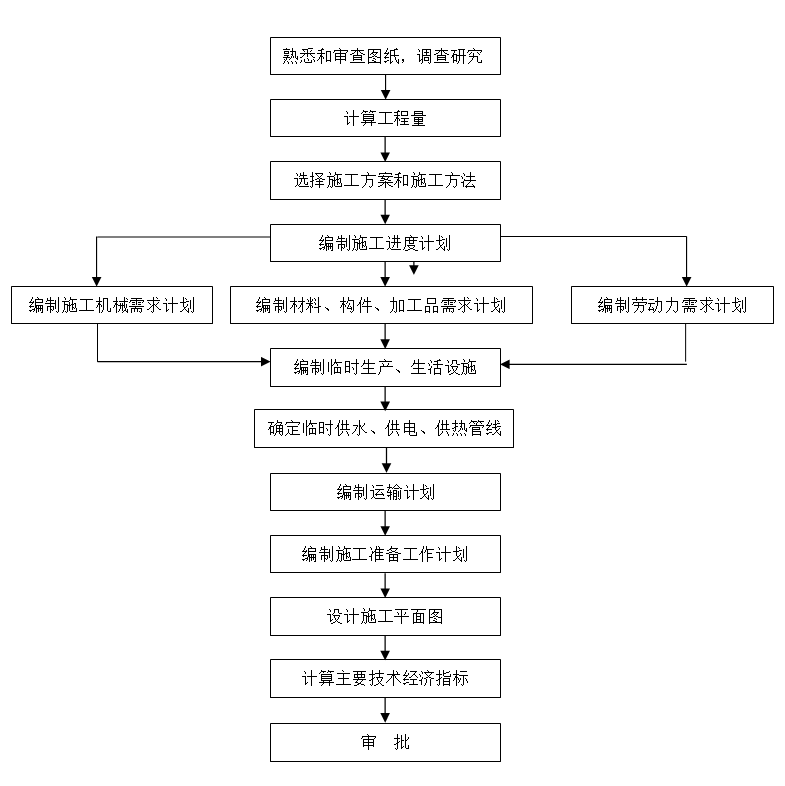
\includegraphics[width=1.0\linewidth]{figure/c1f1.png}
    \caption{单位工程施工组织设计编制程序}
    \label{fig:c1f1}
\end{figure}

\subsection{指导方针及编制依据}

\subsubsection{指导方针}

(1) 主要指导方针\\

为保证在计划工期内圆满地完成施工任务,本施工组织设计的主要指导方针是“服务至上,质量争先,科技先导,管理一流”。\\

(2) 科学组织、精心施工\\

组建一个高效团结的工程项目部和一支技术熟练、作风过硬的施工队伍,运用先进科学的现代化管理手段,
调动企业人力、物力、机械设备等各方面的优势资源,精心组织,与甲方、监理、各专业施工单位、工种密切配合,
根据工期进度要求,从图纸设计、现场测量、材料组织、现场施工、质量检验实行流水节拍式循环作业,
确保工程顺利按时完工。\\

(3) 质量第一、安全至上\\

制定严格的质量保证制度,充分考虑国家现行有关施工质量验收规范、标准和规定的要求,
从人员、材料、机械、环境等方面采取保证质量的措施,实施全员质量管理,确保工程质量达到预定目标。
建立完善的安全保证体系,制定严格的安全管理制度,遵守有关施工安全、防火、环卫的法律、法规,
坚决杜绝重大伤亡事故的发生,保证安全施工、文明施工。\\

(4) 科技先导、争创一流\\

采用先进的施工技术,科学合理地确定施工方案,在确保施工质量和效果的前提下,提高材料利
用率和工作效率,降低施工成本,提高经济效益。

\subsubsection{编制依据}

施工组织设计应以下列内容为主要编制依据:

\begin{itemize}

    \item [1)] 与建筑工程有关的法律、法规和相关文件;

    \item [2)] 国家现行有关标准、规范和技术经济指标;

    \item [3)] 工程所在地的行政主管部门的管理要求;

    \item [4)] 建筑施工行业相关的的质量、环境、职业健康安全管理体系管理规范的要求;

    \item [5)] 工程施工合同及招投标文件;

    \item [6)] 工程设计文件;

    \item [7)] 项目周边环境、现场条件、工程地质和水文、气象等自然条件;

    \item [8)] 与工程项目施工有关的资源供应、生产要素配置情况;

    \item [9)] 施工单位的生产能力、机具设备状况、技术水平等等。
    
\end{itemize}

\subsection{工程概况}
\subsubsection{建筑设计概况}

本工程名称为河南省旅游服务中心,建设地点为河南省郑州市,用地面积为 33333 平方米,总建筑面积为 29175 平方米,其中地上建筑面积 21332 平方米,其中地上建筑面积
地下建筑面积为 7843 平方米,建筑占地面积 8116 平方米,建筑高度 36 米,地上五层,地下一层;本工程为一类高层
建筑,建筑耐火等级为一级,设计使用年限为 50 年。

\subsubsection{结构设计概况}

本工程建造于河南省郑州市郑东新区,拟建层数地上五层,地下一层,主体结构高度 32.25m。
本工程的结构性质为 A 级高度高层建筑,结构体系为钢筋硂框架——剪力墙结构,使用年限 50 年
安全等级二级,主体结构采用桩基,设计等级甲级,基础安全等级二级。结合本工程所处地理位置,建筑
抗震设防类别为丙类,抗震设防烈度为 7 度。

\subsection{气象地质特点}
\subsubsection{气象特点}

郑州市位于河南省中部地区, 属暖温带亚湿润季风气候。四季分明,雨热同期,干冷同季。随着四季更替,依次呈现春季干旱少雨,
夏季炎热多雨,秋季晴朗日照长,冬季寒冷少雨雪的基本气候特征。年平均气温 14.3° C,7 月最热,平均 27°C;1 月最冷,
平均 0.1°C;年平均降雨量 632 毫米,无霜期 220 天,全年日照时间约 2400 小时。适宜的温度条件,充足的光照和农作物生长季节较为丰沛的雨量,构成了良好的农业气象条件。

\subsubsection{地质特点}

郑州市,位于东经 112°42'-114°13' ,北纬 34°16'-34°58',山地面积约 2377 平方公里, 水面面积约 11.4 平方公里。郑州北临黄河,西依嵩山,东南为广阔的黄淮平原,
东面是七朝古都东京开封市,西面为十三朝古都洛阳市,南面是许昌市,北面为焦作市和新乡市。郑州市横跨中国二、三级地貌台阶,西南部嵩山属第二级地貌台阶前缘,
东部平原为第三级地貌台阶的组成部分,山地与平原之间是低山丘陵地带。郑州最高点位于登封市的少室山,连天峰海拔约 1512.4 米;最低点位于中牟县韩寺镇胡辛庄,
海拔73米。邙山位于郑州市西北隅,邙山的地貌主要为黄土台地和黄土丘陵,由于黄河的侧蚀和众多沟谷侵蚀作用,使得黄土丘陵形态显得异常陡峻。

郑州地区位于丘陵岗地与泛滥平原相交接地带,为华北的平原一部分。地形比较平坦,地势由西南向东北倾斜。郑州区内地貌类型复杂多样,按其形态区内地貌依次分为:
丘陵岗地,波状平原,倾斜平原及泛滥平原。
\section{施工组织设计}
\subsection{施工流向、程序及顺序}
\subsubsection{施工流向}
\subsubsection{施工程序}
\subsubsection{施工顺序}
\subsection{施工组织机构及主要管理人员职能}
\subsubsection{施工组织机构}
\subsubsection{主要管理人员职责}
\subsection{施工总平面布置说明}
\subsubsection{现场道路}
\subsubsection{现场材料堆放}
\subsubsection{现场垂直运输系统}
\subsubsection{现场用电布置}
\subsubsection{现场临时设施}
\subsection{施工总进度计划及工期保证措施}
\subsubsection{整体工期控制目标}
\subsubsection{主要施工程序进度计划控制}
\subsubsection{工期保证措施}
\subsection{主要项目施工方法和技术措施}
\subsubsection{土方开挖工程}
\subsubsection{土方回填工程}
\subsubsection{钢筋工程}
\subsubsection{模板及支撑工程}
\subsubsection{混凝土工程}
\subsubsection{脚手架工程}
\subsubsection{砌体工程}

\section{危险因素辨识与评价}

\subsection{危险因素辨识目的和范围}

根据规范《重大危险源辨识》(GB 18218-2018),所谓重大危险源就是指长期或临时地生产、加工、搬运或贮存危险物质,
且危险物质的数量等于或大于临界量的单元对于路桥工程施工过程中,对于重大危险源的界定主要包括:
人的危险行为及管理的漏洞、物的不安全的状态、恶劣的环境影响等,由于建筑施工现场的复杂性,工程施工事故可能随时发生,
并可导致人员死亡及伤害、破坏、财产损失,这对于建筑施工工程的整体施工进度已经企业的经济效益都会造成恶劣的影响,
甚至危及企业的发展,因此建筑施工过程中对于重大危险源的辨识、评价和控制,就显得格外重要。

对于重大危险源的辨识,可根据对危险源危险等级的评定方法进行,一般是对施工过程中危险源带来的风险进行评价分析,
根据评价结果又针对性地进行风险控制,从而达到持续改进的目的。常用的风险评价方法有:
作业条件危险性评价法(LEC)、矩阵法、预先危害分析 (PHA)、故障类型及影响分析 (FMEA)、风险概率评价法 (PRA)、危险可操作性研究 (HAZOP)、事故树分析 (ETA) 等等。

\subsection{危险源辨识}
\subsubsection{基坑工程危险源辨识}
\subsubsection{钢筋工程危险源辨识}

\quan{1} 钢筋加工操作人员未经过相关技术交底和培训,不了解钢筋加工机械的操作方法,导致钢筋加工过程中造成机具伤害;

\quan{2} 钢筋作业人员未取得从业资格证件,无特种作业操作证,在焊接过程中误操作导致触电或者火灾;

\quan{3} 预应力钢筋材料进场未经过检验,导致材料不合格;

\quan{4} 钢筋加工机械未经检验或未按时保养,造成在使用过程中造成触电;

\quan{5} 当使用卷扬机进行冷拉操作时,由于卷扬机固定未有妥善导致被拔出而造成的物体打击;或是卷扬机钢丝绳破损而造成的伤害;

\quan{6} 钢筋切断机锯盘无安全防护导致的机械伤害;

\quan{7} 由于未控制钢筋的冷拉率而造成的的超拉现象,导致机械伤害;

\quan{8} 采用切割机进行切割作业时由于无挡板造成火星飞溅而引起火灾;

\quan{9} 带电操作时未执行“一机一闸一箱一漏”的管理规定而导致储电;

\subsubsection{模板工程危险源辨识}
\subsubsection{混凝土工程危险源辨识}
\subsubsection{脚手架工程危险源辨识}

\quan{1} 由于连墙件未按规定搭设、随意拆除、搭设位置或搭设结构不合理而造成的架体倾倒

\quan{2} 由于基础发生严重破坏或地基不均匀沉降而造成的架体倾倒

\quan{3} 由于脚手架设计承载力不足而造成超载而引发的架体倾倒

\quan{4} 由于脚手架作业成没有铺设妥善脚手板,或者是架体边缘的空隙过大而引发的高处坠落

\quan{5} 由于作业人员高空抛物而造成的物体打击或是高处坠落

\quan{6} 脚手架上随意堆放物品而造成的物体打击

\quan{7} 工人作业未有佩戴防护措施而造成的物体打击或高处坠落

\subsubsection{吊装作业危险源辨识}

\quan{1} 起重机在运行中对人体造成的挤压或撞击;

\quan{2} 起重机吊钩超载断裂、吊运时钢丝绳从吊钩中滑出;

\quan{3} 吊运中重物坠落造成物体打击,重物从空中落到地面又反弹伤人;

\quan{4} 钢丝绳或麻绳断裂造成重物下落;使用应报废的钢丝绳,使用的吊具吊运超过额定起重量的重物等造成重物下落;

\quan{5} 汽车起重机作业场所地面不平整、支撑不稳定、配重不平衡、重物超过额定起重量而造成起重机倾覆;

\quan{6} 风力过大、违章作业造成起重机倾覆;

\quan{7} 机械传动部分未加防护,造成机械伤害;违章在卷扬机钢丝绳上面通过,运动中的钢丝绳将人挤伤或绊倒;

\quan{8} 载货升降机违章载人;

\quan{9} 人站在起重臂下等危险区域;

\quan{10} 电气设备漏电、保护装置失效、裸导线未加屏蔽等造成触电;

\quan{11} 人站立或坐在吊钩上;

\quan{12} 吊运时无人指挥、作业区内有人逗留、运行中的起重机的吊具及重物摆动撞击行人;

\quan{13} 起重工及其他操作人员未戴安全帽等个人防护用品;

\quan{14} 司机视野不清、与指挥人员联络不畅,或误解吊运信号;

\quan{15} 吊挂方式不正确,造成重物从吊钩中脱出;

\quan{16} 使用的钢丝绳超过安全系数;

\quan{17} 钢丝绳从滑轮中跳出轮槽;

\quan{18} 制动器出现裂纹、摩擦垫片磨损过多;

\subsubsection{其他工程危险源辨识}
\subsection{安全评价}
\subsubsection{评价依据}
\subsubsection{评价目的与评价范围}
\subsubsection{安全评价方法}
\subsubsection{评价单元的划分}
\subsubsection{基坑坍塌事故故障树法安全分析}
\subsubsection{模板工程坍塌事故故障树法安全分析}
\subsubsection{高处坠落事故故障树法安全分析}
\subsubsection{物料提升机与施工升降机安全检查表法安全分析}
\subsubsection{施工用电安全检查表法安全分析}
\subsubsection{脚手架工程预先危害分析法安全分析}
\section{第四章}

\section{模板工程专项安全施工方案}
\subsection{编制依据}

\subsection{工程概况}

\subsection{模板支撑架搭设要求}

\subsection{模板计算书}
\subsubsection{基本参数}

\subsubsection{模板安全性验算}

\subsection{模板安装及拆除}
\subsubsection{模板安装施工工艺}

\subsubsection{模板拆除}

\subsection{模板工程安全措施}

\section{基坑支护结构专项施工方案}
\subsection{编制依据和工程概况}
\subsubsection{编制依据}

\subsubsection{工程概况}

\subsection{支护结构准备}
\subsubsection{灌注桩施工方案}

\subsubsection{锚杆施工方案}

\subsection{支护结构计算}
\subsubsection{混凝土灌注桩计算}

\subsubsection{锚杆设计计算}

\subsection{施工安全保障措施}

\section{施工现场安全管理措施}

\subsection{安全管理方针及目标}
\subsubsection{安全管理方针}

(1) 杜绝人身重伤、死亡责任事故,轻伤负伤率指标控制在 0.3\%;

(2) 确保安全文明标准化工地;

(3) 安全隐患排查整改率 100\%;

(4) 实现无重大设备事故、无重大火灾事故、无重大交通事故、无多人急性中毒事故;

(5) 认真贯彻中国建筑《安全生产管理手册》和《施工现场安全防护标准图册》,施工现场安全防护标准化合格率 100\%;

(6) 安全管理人员持证上岗率 100\%,特种作业管理人员持证上岗率 100\%。

\subsection{现场特种作业安全教育}

根据《安全生产法》、《建筑安全生产管理条例》、国家安全生产监督局第13号令《特种作业人员安全技术培训考核管理办法》,
特种作业人员必须经过专门培训,考试合格获得上岗证后方可进行特种作业操作。\\

(1) 电工安全教育\\

\quan{1} 作业人员,必须经专业技术培训、考试合格,方准上岗独立操作;

\quan{2} 必须穿绝缘鞋,戴好安全帽及防护手套和工作相关的防护用具。携带试电笔,不准使用无绝缘的金属工具,以免造成导线接地,短路及人身触电事故。
工作时严禁用手触摸带电设备及非绝缘部分;

\quan{3} 在施工现场检修机械设备或线路,必须在配电室拉掉相应的控制开关,并悬挂“严禁合闸”的警示牌;

\quan{4} 巡视线路或检修配电子表箱,不论线路是否停电,均视为带电,当发现故障时,应有防止跨步电压及接触电压的措施。
方可进行检修工作;

\quan{5} 对施工现场的配电箱内的漏电保护器要每周进行一次检查;\\


(2) 焊工安全教育\\

\quan{1} 焊接作业人员,必须经专业技术培训、考试合格,方准上岗独立操作。非焊工严禁进行电焊作业;

\quan{2} 操作前应检查所有工具、电焊机、电源开关及线路是否良好,金属外壳应有安全可靠的接地,进出应有完整的防护罩;

\quan{3} 操作时应穿工作服、绝缘鞋和戴电焊手套、防护面罩等安全防护用品。清除作业点周围 10 米范围内的易燃易爆物品;

\quan{4} 高处作业时,必须专人监护、系好安全带,焊工必须站在稳固的操作平台上作业,严禁将焊接电缆挂在脖颈上;

\quan{5} 焊接时二次线必须双线到位,严禁借用金属管道,金属、轨道及结构钢筋作回路地线;

\quan{6} 清除焊渣时,应佩带眼睛式面罩,防止焊渣溅入眼内或烫伤皮肤;

\quan{7} 搬运氧气瓶、乙炔气瓶时,必须装好防振圈,避免碰撞、振动;使用保管中应避免曝晒和火烤,乙炔瓶、氧气瓶及易燃物品等严禁同车运输;

\quan{8} 气瓶使用时,氧气瓶与乙炔气瓶之间不应小于 5m。 氧气瓶、乙炔瓶与切割点、明火安全距离 10 米以上;

\quan{9} 氧气瓶及压力表的部位,均不得沾染油污,不准撞击、滚动和曝晒。氧气表和乙炔表冻结时,不准用火烤或锤打,应使用热水或蒸汽解冻。 \\

(3) 铲车司机安全教育\\

\quan{1} 作业前应检查发动机的油、水应加足,各操纵杆放在空挡位置,制动灵敏可靠,灯光仪表齐全、有效方可起动;

\quan{2} 机械起动必须先鸣笛,将铲斗提升离地面 50cm 左右。行驶中可用高速档,但不得进行升降和翻转铲斗动作,作业时应使用低速档,铲斗下方严禁有人,严禁用铲斗载人;

\quan{3} 装载机不得在倾斜的场地上作业,作业区不得有障碍物及无关人员。装卸作业应在平整地面进行;

\quan{4} 向汽车内卸料时,严禁将铲斗从驾驶室顶上越过,铲斗不得碰撞车厢,严禁车厢内有人,不得用铲斗运物料;

在沟槽边卸料时,必须设专人指挥,装载机前轮应与沟槽边缘保持不少于 2m 的安全距离,并放置挡木挡掩;

\quan{5} 将大臂升起进行维护、润滑时,必须将大臂支撑稳固;

\quan{6} 作业后应将装载机开至安全地区,不得停在坑洼积水处,必须将铲斗平放在地面上,将手柄放在空挡位置,拉好手制动器。关闭门窗加锁后,方可离开。\\

(4) 挖掘机机操作员安全教育\\

\quan{1} 挖掘机司机必须经专业技术培训,考试合格取证后方可上
车独立操作。司机应熟知挖掘机的机械原理,保养规则,安全操作规程,并要按规定严格执行。严禁酒后或身体不适时进行操作;

\quan{2} 挖掘机在工作前,应向施工人员了解施工条件和任务。挖掘机进入现场后,司机应遵守施工现场的有关安全规则;

\quan{3} 挖掘机在工作前,应按照日常例行保养项目,对挖掘机进行检查、保养、调整、紧固。挖掘机在工作中,严禁进行维修、保养、紧固等工作。工作过程中若发生异响、异味、温升过高等情况,应立即停车检查;

\quan{4} 挖掘机工作时应当处于水平位置,并将走行机构刹住。若地面泥泞、松软和有沉陷危险时,应用枕木或木板垫妥;

\quan{5} 若必须在挖掘机回转半径内工作时,挖掘机必须停止回转,并将回转机构刹住后,方可进行。同时,机上机下人员要彼此照顾,密切配合,确保安全;

\quan{6} 挖掘机装载活动范围内,不得停留车辆和行人。若往汽车上卸料时,应等汽车停稳,驾驶员离开驾驶室后,方可回转铲斗,向车上卸料。挖掘机回转时,
应尽量避免铲斗从驾驶室顶部越过。卸料时,铲斗应尽量放低,但又注意不得碰撞汽车的任何部位;

\quan{7} 挖掘机回转时,应用回转离合器配合回转机构制动器平稳转动,禁止急剧回转和紧急制动;

\quan{8} 铲斗未离开地面前,不得做回转、走行等动作。铲斗满载悬空时,不得起落臂杆和行走;

\quan{9} 挖掘机不论是作业或走行时,都不得靠近架空输电线路。如必须在高低压架空线路附近工作或通过时,机械与架空线路的安全距离,必须符合规定尺寸。雷雨天气,严禁在架空高压线近旁或下面工作。
在地下电缆附近作业时,必须查清电缆的走向,并用白粉显示在地面上,并应保持1米以外的距离进行挖掘;

\quan{10} 夜间工作时,作业地区和驾驶室,应有良好的照明;

\quan{11} 挖掘机工作后,应将机械驶离工作地区,放在安全、平坦的地方。将机身转正,使内燃机朝向阳方向,铲斗落地,
并将所有操纵杆放到“空档”位置,将所有制动器刹死,关闭发动机。按照保养规程的规定,做好例行保养。关闭门窗并上锁后,方可离开;

\quan{12} 挖掘机装卸车时,应由专人指挥。装卸过程中,挖掘机在坡道上严禁回转或转向。装车时若发生危险情况,可将铲斗放下,协助制动,然后挖掘机缓缓退下。\\

(5) 起重机械操作员安全教育\\

\quan{1} 起重指挥应由技术熟练、懂得起重机械性能、经过专业培训的人员担任,持证上岗。指挥时应站在能够照顾到全面工作的地点,所发信号应事先统一,并做到准确、清楚;

\quan{2} 所有人员严禁在起重臂和吊起的重物下面停留或行走;

\quan{3} 起吊物件应使用交互捻制的钢丝绳。钢丝绳如有扭结、变形,断丝、锈蚀等异常现象,应及时降低使用标准或报废;

\quan{4} 钢丝绳中有一整股折断时、断丝数目在使用中增加很快时,该绳应立即更换。钢丝绳有明显的内部腐蚀时、钢丝绳局部外层钢丝伸长呈笼形态时,应立即报废。\\

\subsection{安全生产管理制度}
\subsubsection{安全教育制度}

\subsubsection{消防安全管理制度}

(1) 消防安全管理责任制

项目消防负责人是工地防火安全的第一责任人,负责本工地的消防安全,主要职责有:\\

\quan{1} 制定并落实消防安全责任制和防火安全管理制度,组织编制火灾的应急预案和落实防火、灭火方案以及火灾发生时应急预案的实施。

\quan{2} 对职工进行消防安全教育,组织消防知识学习,使职工懂得安全动火、用电和其他防火、灭火常识,增强职工消防意识和自防自救能力。

\quan{3} 组织火灾自救,保护火灾现场,协助火灾原因调查

\quan{4} 要掌握单位内重点部位生产储存物资的性质和灭火器材的分布情况,会使用灭火器材扑灭初起火灾。\\

(2) 施工现场三级动火管理制度\\

\quan{1} 一级动火审批制度:在禁火区域内,密闭的室内、施工现场进行动火作业,由动火部门填写动火申请表,由现场管理人员
进行检查,上报公司和上级主管部门进行核查后方可动火;

\quan{2} 在具有一定危险因素的非禁火区域进行临时焊接作业,或是在节假日期间动火,由项目负责人填写动火许可证,并附上
技术方案,经现场管理人员检查无误后上报公司安全部门,批准后方可动火;

\quan{3} 在非固定的、无危险因素的场所进行动火作业,由申请动火者填写动火申请单,经现场安全负责人审查无误后,方可动火。\\

(3) 消防器材与后勤管理制度\\

\quan{1} 在防火要害部位设置的消防器材,由该部位的消防职能人负责维修及保管。

\quan{2} 器材保管人员,应懂得消防知识,正确使用器材,工作认真负责。

\quan{3} 定期检查消防器材,发现超期、缺损的,及时向消防负责人汇报,及时更新;

\quan{4} 对进入仓库的易燃物品要按类存放,并挂设好警示牌和灭火器。

\quan{5} 经常注意季节性变化情况,气温超过 38 摄氏度时,应及时采取措施,防止易燃品自燃起火。\\

(4) 现场生活区防火制度\\

\quan{1} 职工宿舍防火工作由宿舍长负责,其余人共同配合;

\quan{2} 宿舍内严禁使用电热器具

\quan{3} 宿舍内由电工接线完毕后,禁止任何人私自乱拉乱接

\quan{4} 严禁躺在床上吸烟

\quan{5} 职工宿舍每 50$m^2$ 布置一只灭火级别不少于 3A 的灭火器,并定期检查其可靠性。

\quan{6} 宿舍区域安全负责人应保持高度警惕,发现危险因素及时消除隐患。\\

\subsubsection{特种设备安全生产管理制度}

\subsubsection{高空作业安全管理制度}

(1) 高空作业管理目标\\

安全生产目标是企业经济指标的重要组成部分,根据《安全生产法》等法律法规和行业安全管理标准,制订安全生产目标管理制度。

安全与生产、安全与效益是一个整体,当发生矛盾时,必须坚持“安全第一”的原则,遵守职业健康安全法律法规,积极为员工创造适宜的、良好的工作环境,以保护员工的身心健康和职业卫生;
为有效地消除和控制危害,需要建立本质安全的科学观念,预防是最佳的选择。需要推行科学的管理体系,建立安全标准化,实行风险预防型管理,
积极采用先进的技术、工艺和设计,树立所有意外事故和职业病都是可以预防的观念;
安全生产的保障需要人机环境的安全系统协调,从人机环境的综合治理入手,坚持不懈、持续改进,没有最好,只有更好。建立安全标准化,也建立了安全工作的长效机制。\\

(2) 高空作业安全管理规定\\

\quan{1} 审批人员赴高处作业现场,检查确认安全措施后,方可批准高处作业。 从事高处作业的单位必须进行高处作业风险分析,落实安全防护措施,方可施工;

\quan{2} 高处作业人员必须经安全教育,熟悉现场环境和施工安全要求。对患有职业禁忌症和年老体弱、疲劳过度、视力不佳及酒后人员等,不准进行高处作业;

\quan{3} 高处作业前,作业人员应检查确认安全措施落实后,方可施工,否则有权拒绝施工作业;

\quan{4} 高处作业人员要按照规定穿戴劳动保护用品,作业前要检查、作业中要正确使用防坠落用品与登高器具、设备; 

\quan{5} 高处作业应设监护人对高处作业人员进行监护,监护人应坚守岗位。高处作业前,施工单位要制订安全措施;

\quan{6} 不符合高处作业安全要求的材料、器具、设备不得使用。
高处作业所使用的工具、材料、零件等必须装入工具袋,上下时手中不得持物;不准投掷工具、材料及其他物品;易滑动、易滚动的工具、材料堆放在脚手架上时,应采取措施,防止坠落。\\

(3) 高空作业分级\\

凡在离地面两米以上进行的作业,都属于高空作业;\\

\quan{1} 作业高度在2米至5米时,称为一级高处作业;

\quan{2} 作业高度在5米以上至15米时,称为二级高处作业;

\quan{3} 作业高度在15米以上至30米时,称为三级高处作业;

\quan{4} 作业高度在30米以上时,称为特级高处作业。\\

\subsection{安全文明施工措施}
\subsubsection{文明施工管理}

项目文明施工是指保持施工场地整洁、卫生,施工组织科学,施工程序合理的一种施工活动。
实现文明施工,不仅要着重做好现场的场容管理工作,而且还要相应做好现场材料、
设备、安全、技术、保卫、消防和生活卫生等方面的管理工作。
一个工地的文明施工水平是该工地乃至所在企业各项管理工作水平的综合体现。

首先,工程项目在施工准备阶段先编制单位工程《施工组织设计》
,《施工组织设计》中必须编制现场文明施工措施,并经相关部门审核、审批合格后方能组织实施。\\

文明施工应遵守以下项目:

(1) 施工现场要建立文明施工责任制,划分区域,明确管理负责人,实行挂牌制,做到现场清洁整齐;

(2) 施工现场场地平整,道路坚实畅通,有排水措施,基础、地下管道施工完后要及时回填平整,清除积土;临时水电要有专人管理,不得有长流水、长明灯;

(3) 施工现场的临时设施,包括生产、办公、生活用房、仓库、料场、临时上下水管道以及照明、动力线路,要严格按施工组织设计确定的施工平面图布置、搭设或埋设整齐;

(4) 工人操作地点和周围必须清洁整齐,做到活完脚下清,工完场地清,丢洒在楼梯、楼板上的杂物和垃圾要及时清除。严禁损坏污染成品,堵塞管道;

(5) 施工现场不准乱堆垃圾及余物。应在适当地点设置临时堆放点,并定期外运。清运垃圾及流体物品,要采取遮盖防漏措施,运送途中不得遗撒。
建筑物内清除的垃圾渣土,要通过临时搭设的竖井或利用电梯井或采取其他措施稳妥下卸,严禁从门窗口向外抛掷;

(6) 根据工程性质和所在地区的不同情况,采取必要的围护和遮挡措施,并保持外观整洁;

(7) 施工现场严禁居住家属,严禁居民、家属、小孩在施工现场穿行、玩耍;

(9) 施工现场应建立不扰民措施,针对施工特点设置防尘和防噪声设施,夜间施工必须有当地主管部门的批准。

\subsubsection{环境保护}

为加强建设工程施工现场管理,防止因建筑施工对环境的污染,依据《中华人民共和国环境保护法》等有关规定制定本措施,意在在施工过程中有效防治扬尘、
噪声、固体废物和废水等污染环境的情况。根据相关规定施工现场建立环境保护管理体系,责任落实到人,并保证有效运行。
应对施工现场防治扬尘、噪声、水污染及环境保护管理工作进行检查和对职工进行环保法规知识培训考核。按照现场常见的环境污染类别,可将环境保护规定大致分为以下三类:\\

(1) 防治大气污染:\\

\quan{1} 施工现场应采取覆盖、固化、绿化、洒水等有效措施,做到不泥泞、不扬尘。

\quan{2} 遇有四级风以上天气不得进行土方回填、转运以及其他可能产生扬尘污染的施工。  

\quan{3} 施工现场有专人负责环保工作,配备相应的洒水设备,及时洒水,减少扬尘污染。  

\quan{4} 建筑物内的施工垃圾清运必须采用封闭式容器吊运,严禁凌空抛撒。施工现场设密闭式垃圾站,施工垃圾、生活垃圾分类存放。施工垃圾清运时提前适量洒水,并按规定及时清运消纳。  

\quan{5} 土方、渣土和施工垃圾的运输,必须使用密闭式运输车辆,并与持有消纳证的运输单位签定防遗撒、扬尘、乱倒协议书。施工现场出入口处设置洗车池。  

\quan{6} 施工现场混凝土浇注使用预拌混凝土,施工现场装修阶段设置搅拌机的机棚必须封闭,并配备有效的降尘防尘装置。  

\quan{7} 拆除旧有和大临建筑时,随时洒水,减少扬尘污染。渣土要在拆除施工完成之日起三日内清运完毕,并遵守拆除工程的有关规定。  \\

(2) 防治水污染:\\

\quan{1} 搅拌机、混凝土输送泵及运输车辆清洗处设置二级沉淀池,废水不得直接排入市政污水管网,经二次沉淀后用于洒水降尘。  

\quan{2} 现场存放油料、油质脱模剂,必须对库房进行防渗漏处理,储存和使用采取防泄漏措施,防止油料泄漏,污染土壤水体。\\

(3) 防治噪声污染:\\

\quan{1} 施工现场遵照《中华人民共和国建筑施工场界噪声限值》制定降噪措施。建筑施工过程中使用的设备,可能产生噪声污染的,按有关规定向工程所在地的环保部门申报。  

\quan{2} 施工现场的电锯、电刨、搅拌机、固定式混凝土输送泵、大型空气压缩机等强噪声设备搭设封闭式机棚,并尽可能设置在远离居民区的一侧,以减少噪声污染。  

\quan{3} 因生产工艺上要求必须连续作业或者特殊需要时,确需在 22 时至次日 6 时期间进行施工的,在施工前到工程所在地建设行政主管部门提出申请,经批准后方可进行夜间施工,做好周边居民工作。并公布施工期限。  进行夜间施工作业时,应采取措施,最大限度减少施工噪声,采用低噪声震捣棒等方法。
承担夜间材料运输的车辆,进入施工现场严禁鸣笛.装卸材料应做到轻拿轻放,最大限度地减少噪声扰民。  

\quan{4} 施工现场进行噪声值监测,监测方法执行《建筑施工场界噪声测量方法》,噪声值不超过国家或地方噪声排放标准。  

\subsection{安全保障措施}
\subsubsection{基坑工程安全保障措施}

\subsubsection{钢筋工程安全保障措施}

\subsubsection{模板工程安全保障措施}

\subsubsection{混凝土工程安全保障措施}

\subsubsection{砌筑工程安全保障措施}

\subsubsection{脚手架搭拆工程安全保障措施}

\subsubsection{施工用电安全保障措施}

\subsubsection{施工机具安全保障措施}

\section{施工现场事故应急预案}
\subsection{总则}
\subsubsection{编制目的}

\subsubsection{编制依据}

\subsubsection{适用范围}

\subsection{应急组织体系}
\subsubsection{事故应急救援组织体系主要职责}

\subsection{应急响应}
\subsubsection{响应分级}

\subsubsection{响应程序}

\subsubsection{应急资源调配}

\subsubsection{应急救援}

\subsubsection{扩大应急}

\subsection{事故应急处置}
\subsubsection{事故应急处置基本要求}

\subsubsection{二级响应处置措施}

\subsubsection{一级响应处置措施}

\subsubsection{事故应急处置结束}

\subsection{事故后期处置}

\subsection{事故应急保障措施}
\subsubsection{应急队伍保障}

\subsubsection{应急物资装备保障}

\subsubsection{其他保障}

\subsection{应急预案管理}
\subsubsection{应急预案修订与备案}

\subsection{火灾事故应急演练}
\subsubsection{指导思想}

\subsubsection{组织与安排}

\subsubsection{火灾应急演练过程}

\subsubsection{演练总结}

\subsection{施工现场专项应急预案}
\subsubsection{高处坠落事故专项应急救援预案}

\subsubsection{机械伤害事故专项应急救援预案}

\subsubsection{火灾事故专项应急救援预案}

\subsection{应急预案的评审与改进}

%=============  结论  ======================
\begin{center}
    \section*{\zihao{-2}  \textbf{结 ~~ 论}}
    \end{center}
\addcontentsline{toc}{section}{结论}

结论是理论分析和实验结果的逻辑发展,是整篇论文的归宿。结论是在理论分析、试验结果的基础上,
经过分析、推理、判断、归纳的过程而形成的总观点。结论必须完整、准确、鲜明、并突出与前人不同的新见解。

书写格式说明:

标题“结论”选用模板中的样式所定义的“结论”,或者手动设置成字体:黑体,居中,字号:小三,1.5倍行距,段后1行,段前为0行。

结论正文选用模板中的样式所定义的“正文”,每段落首行缩进2字;或者手动设置成每段落首行缩进2字,字体:宋体,字号:小四,行距:多倍行距 1.25,间距:段前、段后均为0行。

%============= 参考文献 =====================
\addcontentsline{toc}{section}{参考文献}
{\zihao{5} \songti \bibliography{bibfile}}
\clearpage
\newpage
\appendix

%=============  致谢  ======================
\begin{center}
    \section*{\zihao{-2}  \textbf{致 ~~ 辞}}
    \end{center}
\addcontentsline{toc}{section}{致辞}

\end{document}
%%%%%%%%%% 结束 %%%%%%%%%%
